%======================================================================
% GMI-07a Asym tenzory.pdf
%======================================================================
% Penroseovy diagramy: krabička s nožičkami
% \gmIsedmAbox{popisek}{seznam koncových poloh nožiček (permutace)}{typ pruhu: 0 nic, 1 antisym., 2 sym.,
%   3 sym. jen nožičky 1-2, 4 antisym. jen nožičky 2-3, 5 = 3 + 4}
\providecommand{\gmIsedmAbox}[3]{%
\begin{tikzpicture}[baseline=(current bounding box.center),x=0.16cm,y=0.16cm,line width=0.5pt]
  \draw (0,-1.6) rectangle (4,0.4); \node[font=\scriptsize] at (2,-0.6) {$#1$};
  \foreach \e [count=\i] in {#2} \draw (\i,0.4) -- (\e,2.6);
  \ifnum#3=1 \draw[line width=1.1pt] (0.5,2.6) -- (3.5,2.6); \fi
  \ifnum#3=2 \draw[decorate,decoration={snake,amplitude=0.4pt,segment length=2pt}] (0.5,2.6) -- (3.5,2.6); \fi
  \ifnum#3=3 \draw[decorate,decoration={snake,amplitude=0.4pt,segment length=2pt}] (0.5,2.6) -- (2.5,2.6); \fi
  \ifnum#3=4 \draw[line width=1.1pt] (1.5,2.6) -- (3.5,2.6); \fi
  \ifnum#3=5 \draw[decorate,decoration={snake,amplitude=0.4pt,segment length=2pt}] (0.5,1.6) -- (2.5,1.6);
             \draw[line width=1.1pt] (1.5,2.6) -- (3.5,2.6); \fi
\end{tikzpicture}}
% antisymetrizační "kartáč" s k nožičkami (projektor)
\providecommand{\gmIsedmAbar}[1]{%
\begin{tikzpicture}[baseline=(current bounding box.center),x=0.16cm,y=0.16cm,line width=0.5pt]
  \foreach \i in {1,2,4} {\draw (\i,-1.4) -- (\i,1.4);}
  \node[font=\tiny] at (3,0.9) {$\cdots$};
  \draw[line width=1.1pt] (0.5,0) -- (4.5,0);
  \draw[decorate,decoration={brace,mirror,amplitude=2pt}] (0.5,-1.8) -- (4.5,-1.8) node[midway,below=1pt,font=\tiny] {$#1$};
\end{tikzpicture}}

\section{Symetrické a antisymetrické tenzory}
\strana{GMI-07a-1}

\begin{itemize}[nosep]
  \item Prostor antisymetrických tenzorů
  \item Vnější součin
  \item Vnitřní součin / AS-dualita
  \item Rozštěpení antisymetrizace
  \item Báze a komponenty AS tenzorů a forem
  \item Totálně antisymetrické tenzory
  \item Determinant
  \item Vnější algebra
  \item Prostor symetrických tenzorů
\end{itemize}

%----------------------------------------------------------------------
\newpage
\strana{GMI-07a-2}
\subsection{Prostor antisymetrických tenzorů}

\[
  V^{[k]}\subset V^k \qquad \dim V^{[k]} = \binom{d}{k} \qquad k = 0,1,\dots,d
\]
\begin{definice}[antisymetrický tenzor]
\[
  A\in V^{[k]} \quad\equiv\quad \forall\sigma \text{ permutace } [1\dots k] \qquad
  A^{a_1\dots a_k} = \operatorname{sign}\sigma\, A^{a_{\sigma 1}\dots a_{\sigma k}}
\]
\end{definice}

\kw{antisymetrizace}
\[
  A = \mathcal{A}B \qquad
  \vzorec{A^{a_1\dots a_k} = B^{[a_1\dots a_k]} = \frac{1}{k!}\sum_\sigma\operatorname{sign}\sigma\,B^{a_{\sigma 1}\dots a_{\sigma k}}}
\]
\[
  \gmIsedmAbox{A}{1,2,3}{0} = \gmIsedmAbox{B}{1,2,3}{1}
  = \frac16\Big(\gmIsedmAbox{B}{1,2,3}{0} + \gmIsedmAbox{B}{2,3,1}{0} + \gmIsedmAbox{B}{3,1,2}{0}
  - \gmIsedmAbox{B}{1,3,2}{0} - \gmIsedmAbox{B}{2,1,3}{0} - \gmIsedmAbox{B}{3,2,1}{0}\Big)
\]
\[
  A\in V^{[k]} \quad\Longleftrightarrow\quad A^{a_1\dots a_k} = A^{[a_1\dots a_k]}
  \qquad\qquad \gmIsedmAbox{A}{1,2,3}{1} = \gmIsedmAbox{A}{1,2,3}{0}
\]
\pozn{v originále diagramy s obecným počtem nožiček}

\begin{vysvetleni}[jak číst diagramy „krabička s nožičkami“]
Jde o variantu Penroseovy grafické notace:
\begin{itemize}[nosep,leftmargin=1.2em]
  \item krabička s popiskem ($A$, $B$, \dots) = tenzor; každá nožička = jeden index, sloty se čtou zleva doprava (nožičky nahoru = horní indexy $a_1a_2a_3$);
  \item zkřížené nožičky = permutace indexů: nožička vycházející z $i$-tého slotu tenzoru končí na pozici, kde stojí volný index, který do slotu dosazujeme. Např.\ \gmIsedmAbox{B}{2,1,3}{0} je $B^{a_2a_1a_3}$;
  \item tlustý vodorovný pruh přes nožičky = antisymetrizace přes ty indexy (hranaté závorky $[\dots]$), vlnovka = symetrizace (kulaté závorky $(\dots)$);
  \item nožičky bez krabičky = Kroneckerova delta (identita), spojení nožičky jednoho objektu s nožičkou druhého = zúžení.
\end{itemize}
Rozepsání pruhu přes 3 nožičky tedy dává všech $3!=6$ permutací, cyklické se znaménkem $+$ a transpozice se znaménkem $-$, s faktorem $\frac1{3!}$. Krtouš diagramy nepoužívá; antisymetrizace viz odd.~1.4, def.~D1.1, D1.2.
\end{vysvetleni}

\kw{projektor} na $V^{[k]}$
\[
  {}^{[k]}\delta\in V^{[k]}_{[k]} \qquad
  {}^{[k]}\delta^{a_1\dots a_k}_{b_1\dots b_k} = \delta^{[a_1}_{b_1}\cdots\delta^{a_k]}_{b_k}
  = \delta^{a_1}_{[b_1}\cdots\delta^{a_k}_{b_k]}
  \qquad\qquad \gmIsedmAbar{k}
\]
\[
  A^{[a_1\dots a_k]} = {}^{[k]}\delta^{a_1\dots a_k}_{m_1\dots m_k}A^{m_1\dots m_k}
  \qquad\qquad \gmIsedmAbox{A}{1,2,3}{1}
\]

\begin{veta}[vlastnosti]
${}^{[k]}\delta$ je projektor
\[
  {}^{[k]}\delta^{a_1\dots a_k}_{m_1\dots m_k}\,{}^{[k]}\delta^{m_1\dots m_k}_{b_1\dots b_k}
  = {}^{[k]}\delta^{a_1\dots a_k}_{b_1\dots b_k}
  \qquad\qquad {}^{[k]}\delta^{m_1\dots m_k}_{m_1\dots m_k} = \dim V^{[k]}
\]
\[
  {}^{[k]}\delta^{a_1\dots a_{k-l}\,m_1\dots m_l}_{b_1\dots b_{k-l}\,n_1\dots n_l}\;
  {}^{[l]}\delta^{n_1\dots n_l}_{b_{k-l+1}\dots b_k}
  = {}^{[k]}\delta^{a_1\dots a_{k-l}\,m_1\dots m_l}_{b_1\dots\dots b_k}
\]
\[
  {}^{[k]}\delta^{a_1\dots a_l\,m_{l+1}\dots m_k}_{b_1\dots b_l\,m_{l+1}\dots m_k}
  = \vzorec{\frac{(d-l)!\,l!}{(d-k)!\,k!}}\;{}^{[l]}\delta^{a_1\dots a_l}_{b_1\dots b_l}
\]
\[
  {}^{[k]}\delta^{a_{\sigma 1}\dots a_{\sigma k}}_{b_{\sigma 1}\dots b_{\sigma k}} = {}^{[k]}\delta^{a_1\dots a_k}_{b_1\dots b_k}
\]
\end{veta}
\begin{center}
\begin{tikzpicture}[x=0.3cm,y=0.3cm,line width=0.5pt]
  % k-bar + l-bar on subset = k-bar
  \foreach \x in {0,1.5,3,4.5,6} \draw (\x,-1.5) -- (\x,1.5);
  \draw[line width=1.2pt] (-0.4,0) -- (6.4,0);
  \draw[line width=1.2pt] (2.6,0.9) -- (6.4,0.9);
  \draw[decorate,decoration={brace,amplitude=3pt}] (2.6,1.8) -- (6.4,1.8) node[midway,above=2pt] {\small $l$};
  \draw[decorate,decoration={brace,mirror,amplitude=3pt}] (-0.4,-1.9) -- (6.4,-1.9) node[midway,below=2pt] {\small $k$};
  \node at (8,0) {$=$};
  \foreach \x in {9.5,11,12.5,14,15.5} \draw (\x,-1.5) -- (\x,1.5);
  \draw[line width=1.2pt] (9.1,0) -- (15.9,0);
  \draw[decorate,decoration={brace,mirror,amplitude=3pt}] (9.1,-1.9) -- (15.9,-1.9) node[midway,below=2pt] {\small $k$};
  % stopa
  \begin{scope}[xshift=7.8cm]
    \foreach \x in {0,1.5,3,4.5,6} \draw (\x,-1.5) -- (\x,1.5);
    \draw[line width=1.2pt] (-0.4,0) -- (6.4,0);
    \draw[rounded corners=2pt] (3,1.5) -- (3,2.1) -- (7,2.1) -- (7,-2.1) -- (3,-2.1) -- (3,-1.5);
    \draw[rounded corners=2pt] (4.5,1.5) -- (4.5,1.8) -- (6.6,1.8) -- (6.6,-1.8) -- (4.5,-1.8) -- (4.5,-1.5);
    \draw[decorate,decoration={brace,amplitude=3pt}] (-0.4,2.4) -- (1.9,2.4) node[midway,above=2pt] {\small $l$};
    \draw[decorate,decoration={brace,mirror,amplitude=3pt}] (-0.4,-2.5) -- (7,-2.5) node[midway,below=2pt] {\small $k$};
    \node at (9.5,0) {$= \dfrac{(d-l)!\,l!}{(d-k)!\,k!}$};
    \foreach \x in {12.5,14} \draw (\x,-1.5) -- (\x,1.5);
    \draw[line width=1.2pt] (12.1,0) -- (14.4,0);
    \draw[decorate,decoration={brace,mirror,amplitude=3pt}] (12.1,-1.9) -- (14.4,-1.9) node[midway,below=2pt] {\small $l$};
  \end{scope}
\end{tikzpicture}
\end{center}
\pozn{indexy ve druhém vztahu (pohlcení menšího projektoru) jsou v originále špatně čitelné; zapsáno podle diagramu}

\begin{vysvetleni}[projektor ${}^{[k]}\delta$ a jeho vlastnosti]
${}^{[k]}\delta$ je „samotný pruh“ přes $k$ svislých čar (čáry = $\delta$): přiložením k libovolnému tenzoru ho antisymetrizuje. Vlastnosti v diagramech:
\begin{itemize}[nosep,leftmargin=1.2em]
  \item dva pruhy za sebou = jeden pruh (antisymetrizovat podruhé nic nemění), $\mathcal{A}^2=\mathcal{A}$;
  \item menší pruh přes část čar je pohlcen větším (antisymetrizace v podmnožině indexů je obsažena v úplné);
  \item stopa (zúžení horního indexu s dolním) = čára uzavřená do smyčky (obrázek vpravo). Kontrola koeficientu: pro $l=0$ dává $\frac{d!}{(d-k)!\,k!}=\binom dk=\dim V^{[k]}$, pro $l=k$ dává $1$.
\end{itemize}
Viz Krtouš, def.~D1.3 a lemma V1.2 (tam jsou stejné vztahy (i)--(vi)).
\end{vysvetleni}

%----------------------------------------------------------------------
\strana{GMI-07a-3}
\subsection{Vnější součin}

\begin{definice}[vnější součin]
\[
  \alpha^j\in V_{[p_j]} \qquad \textstyle\sum p_j = p
\]
\[
  \vzorec{\alpha^1\wedge\dots\wedge\alpha^k = \frac{p!}{p_1!\cdots p_k!}\,\mathcal{A}(\alpha^1\dots\alpha^k)}
\]
\[
  (\alpha^1\wedge\dots\wedge\alpha^k)_{e_1\dots e_p} = \frac{p!}{p_1!\cdots p_k!}\,
  \alpha^1_{[e_1\dots}\alpha^2_{e_{p_1+1}\dots}\cdots\alpha^k_{\dots e_p]}
\]
\end{definice}

\begin{veta}[vlastnosti]
\begin{align*}
  (\alpha\wedge\beta)\wedge\gamma &= \alpha\wedge\beta\wedge\gamma && \text{asociativita} \\
  \underset{p}{\alpha}\wedge\underset{q}{\beta} &= (-1)^{pq}\,\beta\wedge\alpha && \text{skew-komutat.}
\end{align*}
\end{veta}
\begin{priklad}[Př.]
$\alpha,\beta$ 1-formy, \ $\sigma$ 2-forma, \ $\omega$ $p$-forma
\[
  \alpha\wedge\beta = -\beta\wedge\alpha \qquad \alpha\wedge\omega = (-1)^p\omega\wedge\alpha \qquad
  \sigma\wedge\omega = \omega\wedge\sigma
\]
\end{priklad}

\begin{vysvetleni}[normalizace vnějšího součinu]
Faktor $\frac{p!}{p_1!\cdots p_k!}$ je zvolen tak, aby se ve výsledku každý „kvalitativně různý“ člen vyskytl s koeficientem $\pm1$ (žádné $\frac12$ apod.): např.\ $\alpha\wedge\beta=2\mathcal{A}(\alpha\beta)=\alpha\beta-\beta\alpha$. Díky tomu je $\wedge$ asociativní a báze $e^{k_1}\wedge\dots\wedge e^{k_p}$ má „jednotkové“ komponenty (GMI-07a-7).
Znaménko $(-1)^{pq}$: přehození $\beta$ před $\alpha$ znamená protlačit každý z $q$ indexů přes $p$ indexů, tj.\ $pq$ transpozic. Sudé formy proto komutují se vším.
Viz Krtouš, odd.~4.2, def.~D4.2, vztah (4.1) a marginálie M4.2 (stejná konvence).
\end{vysvetleni}

\kw{normovaná wedge}
\[
  (\alpha^1\wedge\dots\wedge\alpha^k)_{e_1\dots e_p}
  = \sum_{\substack{\text{rozdělení čísel}\\ (1\dots p)\text{ na }K\text{ skupin}\\ \sigma^1\dots\sigma^K\text{ délek }p_1\dots p_K}}
  \operatorname{sign}\sigma\;
  \alpha^1_{e_{\sigma^1_1}\dots e_{\sigma^1_{p_1}}}\,
  \alpha^2_{e_{\sigma^2_1}\dots e_{\sigma^2_{p_2}}}\cdots
  \alpha^K_{e_{\sigma^K_1}\dots e_{\sigma^K_{p_K}}}
\]

\begin{priklad}[Př.]
\begin{align*}
  (\alpha\wedge\beta)_{ab} &= \alpha_a\beta_b - \alpha_b\beta_a & \alpha\wedge\beta &= \alpha\beta - \beta\alpha \\
  (\alpha\wedge\sigma)_{abc} &= \alpha_a\sigma_{bc} + \alpha_b\sigma_{ca} + \alpha_c\sigma_{ab} \\
  (\underset{2}{\omega}\wedge\underset{2}{\sigma})_{abcd} &= \omega_{ab}\sigma_{cd} - \omega_{ac}\sigma_{bd} + \omega_{ad}\sigma_{bc} \\
  &\quad + \omega_{bc}\sigma_{ad} - \omega_{bd}\sigma_{ac} + \omega_{cd}\oprava{\sigma_{ab}}{\beta_{ab}}
\end{align*}
\end{priklad}

\begin{vysvetleni}[součet přes rozdělení indexů]
Indexy $e_1\dots e_p$ rozdělíme do skupin délek $p_1,\dots,p_K$, uvnitř každé skupiny ponecháme rostoucí pořadí („shuffle“); takových rozdělení je $\frac{p!}{p_1!\cdots p_K!}$. Znaménko je znaménko permutace, která seřadí indexy (skupina 1, skupina 2, \dots) zpět na $e_1\dots e_p$.
Kontrola na příkladu dvou 2-forem: rozdělení $\{ab|cd\},\{ac|bd\},\{ad|bc\},\{bc|ad\},\{bd|ac\},\{cd|ab\}$ se znaménky $+,-,+,+,-,+$ -- přesně šest členů výše, $\binom42=6$.
U $(\alpha\wedge\sigma)_{abc}$ jsou členy přepsány pomocí antisymetrie $\sigma$ do cyklického tvaru ($-\alpha_b\sigma_{ac}=\alpha_b\sigma_{ca}$). Srov.\ Krtouš (4.4), kde je tentýž rozpis zapsán s jinak uspořádanými indexy.
\end{vysvetleni}

%----------------------------------------------------------------------
\strana{GMI-07a-4}
\begin{veta}[Theorem]
\[
  \alpha_{\mu_1\dots\mu_s}\wedge\beta_{\mu_{s+1}\dots\mu_r} =
  \sum_{1\le k_1<k_2<\dots<k_s\le r}(-1)^{k_1+\dots+k_s+\frac{s(s+1)}{2}}\,
  \alpha_{\mu_{k_1}\dots\mu_{k_s}}\,\beta_{\underbrace{\mu_1\dots\mu_r}_{\text{mimo }\mu_{k_1}\dots\mu_{k_s}}}
\]
\end{veta}
Důkaz:
\begin{align*}
  \sum_{1\le k_1<\dots<k_s\le r}&(-1)^{k_1+\dots+k_s+\frac{s(s+1)}{2}}\,
    \alpha_{\mu_{k_1}\dots\mu_{k_s}}\,\beta_{\underbrace{\mu_1\dots\mu_r}_{\text{mimo }\mu_{k_1}\dots\mu_{k_s}}} = \\
  &= \sum_{1\le k_1<\dots<k_s\le r}(-1)^\sigma\,\alpha_{\mu_{\sigma_1}\dots\mu_{\sigma_s}}\,\beta_{\mu_{\sigma_{s+1}}\dots\mu_{\sigma_r}} =
  \qquad \sigma: \begin{bmatrix} 1 & 2 & \dots & s & s+1 & \dots & r \\
                                k_1 & k_2 & \dots & k_s & \multicolumn{3}{c}{\underbrace{1\ \dots\ r}_{\text{mimo }k_1\dots k_s}} \end{bmatrix} \\
  &= \frac{1}{s!}\frac{1}{(r-s)!}\sum_{\sigma\in P_{1\dots r}}(-1)^\sigma\,\alpha_{\mu_{\sigma_1}\dots\mu_{\sigma_s}}\,\beta_{\mu_{\sigma_{s+1}}\dots\mu_{\sigma_r}} \\
  &= \binom{r}{s}\,\alpha_{[\mu_1\dots\mu_s}\beta_{\mu_{s+1}\dots\mu_r]} = \\
  &= \alpha_{\mu_1\dots\mu_s}\wedge\beta_{\mu_{s+1}\dots\mu_r}
\end{align*}

\begin{veta}[Theorem]
\begin{align*}
  \alpha_{\mu_0}\wedge\beta_{\mu_1\dots\mu_r} &= \sum_{0\le k\le r}(-1)^k\,\alpha_{\mu_k}\,
    \beta_{\underbrace{\mu_0\dots\mu_r}_{\text{mimo }\mu_k}} \\
  \alpha_{\mu_1\mu_2}\wedge\beta_{\mu_3\dots\mu_r} &= \sum_{1\le k<l\le r}(-1)^{k+l+1}\,\alpha_{\mu_k\mu_l}\,
    \beta_{\underbrace{\mu_1\dots\mu_r}_{\text{mimo }k,l}}
\end{align*}
\end{veta}

\begin{vysvetleni}[indexový zápis $\wedge$ a znaménko]
Indexy psané u jednotlivých činitelů ($\alpha_{\mu_1\dots\mu_s}\wedge\beta_{\mu_{s+1}\dots\mu_r}$) jen naznačují sloty výsledné $r$-formy -- jde o komponentu $(\alpha\wedge\beta)_{\mu_1\dots\mu_r}$.
Permutace, která přesune pozice $k_1<\dots<k_s$ dopředu a zbytek ponechá v pořadí, má znaménko $(-1)^{\sum_i(k_i-i)}=(-1)^{k_1+\dots+k_s-\frac{s(s+1)}2}$, což je totéž jako $(-1)^{k_1+\dots+k_s+\frac{s(s+1)}2}$, protože $s(s+1)$ je sudé. V důkazu se součet přes $s!\,(r-s)!$ permutací uvnitř skupin „schová“ do antisymetrie $\alpha$ a $\beta$.
Pro $s=1$ (indexy od $0$) dostaneme $(-1)^k$, pro $s=2$ $(-1)^{k+l+3}=(-1)^{k+l+1}$. Viz Krtouš, marginálie M4.2, vztah (4.3) a dodatek 4.A.
\end{vysvetleni}

%----------------------------------------------------------------------
\strana{GMI-07a-5}
\subsection{Vnitřní součin / AS-dualita}

\begin{definice}[vnitřní součin]
\[
  \circ:\ V_{[k]}\times V^{[k]}\to\mathbb{R}
\]
\[
  \vzorec{\omega\circ w = \frac{1}{k!}\,\mathcal{C}^{\text{vše}}\,\omega w = \frac{1}{k!}\,\omega_{a_1\dots a_k}w^{a_1\dots a_k}}
\]
zobecnění na $V_{[k]}\times V^{[l]}$ \ -- suma přes všechny indexy, co jsou k dispozici
\end{definice}

\kw{zúžení s vektorem}
\[
  u\cdot\omega \equiv u\,\lrcorner\,\omega = \iota_u\omega = u\circ\omega
  \qquad\qquad (u\cdot\omega)_{e_1\dots} = u^a\omega_{ae_1\dots}
\]

\begin{vysvetleni}[proč $\frac1{k!}$ ve vnitřním součinu]
V plném zúžení $\omega_{a_1\dots a_k}w^{a_1\dots a_k}$ se každá nezávislá komponenta (s $a_1<\dots<a_k$) objeví $k!$-krát se stejnou hodnotou součinu. Faktor $\frac1{k!}$ to kompenzuje: $\omega\circ w=\sum_{a_1<\dots<a_k}\omega_{a_1\dots a_k}w^{a_1\dots a_k}$, a báze $e^{k_1\dots k_p}$, $e_{l_1\dots l_p}$ jsou pak navzájem duální (GMI-07a-7).
Při zúžení s vektorem ($l=1$) je faktor $\frac1{1!}=1$, takže $u\cdot\omega=\iota_u\omega$ je prosté dosazení $u$ do \emph{prvního} slotu formy. Pro 1-formu $u\cdot\alpha=u^a\alpha_a$ je číslo, pro funkci (0-formu) je $\iota_uf=0$.
\end{vysvetleni}

\begin{veta}[zúžení je (alg.) derivace vůči $\wedge$]
\[
  \vzorec{u\cdot(\underset{p}{\alpha}\wedge\underset{q}{\beta}) = (u\cdot\alpha)\wedge\beta + (-1)^p\alpha\wedge(u\cdot\beta)}
\]
\begin{align*}
  u\cdot(\alpha^1\wedge\alpha^2\wedge\alpha^3\wedge\dots) = \ &(u\cdot\alpha^1)\wedge\alpha^2\wedge\alpha^3\wedge\dots
    + (-1)^{p_1}\alpha^1\wedge(u\cdot\alpha^2)\wedge\alpha^3\wedge\dots \\
  &+ (-1)^{p_1+p_2}\alpha^1\wedge\alpha^2\wedge(u\cdot\alpha^3)\wedge\dots + \dots
\end{align*}
\end{veta}

\textbf{jednoznačnost operace}

\begin{veta}[Tvrzení]
operace $\iota_a$ na formách splňující
\begin{align*}
  &\iota_a(\omega + \sigma) = \iota_a\omega + \iota_a\sigma \\
  &\iota_a(\omega\wedge\sigma) = (\iota_a\omega)\wedge\sigma + (-1)^p\omega\wedge\iota_a\sigma \\
  &\iota_af = 0 && f \text{ 0-forma} \\
  &\iota_a\alpha = a\cdot\alpha && \alpha \text{ 1-forma}
\end{align*}
je už jednoznačně určená
\[
  \iota_a\omega = a\cdot\omega
\]
$\Leftarrow$ rozklad obecné $\omega$ na elementární členy
\end{veta}

\begin{vysvetleni}[$\iota_u$ jako antiderivace]
$\iota_u$ snižuje stupeň o $1$ a Leibnizovo pravidlo má znaménko $(-1)^p$: při „průchodu“ přes $p$-formu $\alpha$ k $\beta$ se musí vektor protlačit přes $p$ indexů. Tím je $\iota_u$ obdobou vnější derivace $d$ (která stupeň zvyšuje) -- obě se kombinují v Cartanově identitě $\mathcal{L}_u=\iota_ud+d\iota_u$ (GMI-06b-6).
Příklad pro 1-formy: $u\cdot(\alpha\wedge\beta)=(u\cdot\alpha)\beta-(u\cdot\beta)\alpha$; přímo z $(\alpha\wedge\beta)_{ab}=\alpha_a\beta_b-\alpha_b\beta_a$ zúžením s $u^a$.
Jednoznačnost: každá forma je součtem vnějších součinů 1-forem (násobených funkcemi) a na nich jsou uvedená pravidla úplným předpisem.
\end{vysvetleni}

%----------------------------------------------------------------------
% čárové diagramy: \gmIsedmAD{počet čar}{další tikz}, \gmIsedmADX = první dvě čáry zkřížené
\providecommand{\gmIsedmAD}[2]{\begin{tikzpicture}[baseline=(current bounding box.center),x=0.17cm,y=0.17cm,line width=0.5pt]
  \foreach \i in {1,...,#1} \draw (\i,-1.3) -- (\i,1.3); #2 \end{tikzpicture}}
\providecommand{\gmIsedmADX}[2]{\begin{tikzpicture}[baseline=(current bounding box.center),x=0.17cm,y=0.17cm,line width=0.5pt]
  \draw (1,-1.3) -- (2,1.3); \draw (2,-1.3) -- (1,1.3);
  \foreach \i in {3,...,#1} \draw (\i,-1.3) -- (\i,1.3); #2 \end{tikzpicture}}
\providecommand{\gmIsedmAas}[3]{\draw[line width=1.1pt] (#1-0.4,#3) -- (#2+0.4,#3);}
\providecommand{\gmIsedmAsy}[3]{\draw[decorate,decoration={snake,amplitude=0.5pt,segment length=2.5pt}] (#1-0.4,#3) -- (#2+0.4,#3);}
\providecommand{\gmIsedmAdots}[1]{\node[font=\tiny] at (#1,-0.8) {$\cdots$};}

\strana{GMI-07a-6}
\subsection{Rozštěpení antisymetrizace}

\begin{align*}
  \alpha_a\wedge\omega_{e_1\dots e_p} &= (p+1)\,\alpha_{[a}\omega_{e_1\dots e_p]} \\
  &= \alpha_a\omega_{e_1\dots e_p} - \alpha_{e_1}\omega_{ae_2\dots e_p} && \to\ -\alpha_{e_1}\omega_{ae_2\dots e_p} \\
  &\phantom{= \alpha_a\omega_{e_1\dots e_p}} - \alpha_{e_2}\omega_{e_1a\dots e_p} && \phantom{\to}\ +\alpha_{e_2}\omega_{ae_1\dots e_p} \\
  &\phantom{= \alpha_a\omega_{e_1\dots e_p}}\ \ \vdots && \phantom{\to}\ \ \vdots \\
  &\phantom{= \alpha_a\omega_{e_1\dots e_p}} - \alpha_{e_p}\omega_{e_1e_2\dots a} && \phantom{\to}\ (-1)^p\alpha_{e_p}\omega_{ae_1\dots e_{p-1}} \\
  &= \vzorec{\alpha_a\omega_{e_1\dots e_p} - p\,\alpha_{[e_1}\omega_{|a|e_2\dots e_p]}}
\end{align*}

\begin{vysvetleni}[rozepsání antisymetrizace přes první index]
Úplnou antisymetrizaci $p+1$ indexů rozepíšeme podle toho, který index „padne“ na $\alpha$ (vztah (4.3) u Krtouše): $\alpha_a\omega_{e\dots}$ a $p$ členů, kde $\alpha$ nese některé $e_i$. Pravý sloupec ($\to$) ukazuje tytéž členy po přesunutí $a$ na první místo ve $\omega$ (každé prohození indexu ve $\omega$ dá znaménko $-$).
Těchto $p$ členů je dohromady $p$-krát antisymetrizace přes $e_1\dots e_p$ výrazu $\alpha_{e_1}\omega_{ae_2\dots e_p}$. Svislé čáry $|a|$ znamenají, že index $a$ se do antisymetrizace nezahrnuje (Krtouš, def.~D1.1).
Diagramy pod tím vyjadřují totéž pro libovolný tenzor, jen bez krabiček.
\end{vysvetleni}

\begin{center}
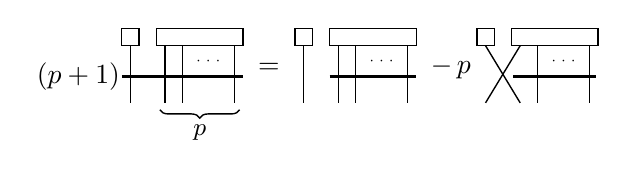
\begin{tikzpicture}[x=0.22cm,y=0.22cm,line width=0.5pt]
  % (p+1) [alpha][omega] s pruhem přes vše
  \node at (-2.5,0) {$(p+1)$};
  \draw (0,1.8) rectangle (1,2.8); \draw (0.5,1.8) -- (0.5,-1.5);
  \draw (2,1.8) rectangle (7,2.8);
  \foreach \x in {2.5,3.5,6.5} \draw (\x,1.8) -- (\x,-1.5);
  \node[font=\tiny] at (5,0.9) {$\cdots$};
  \draw[line width=1.1pt] (0,0) -- (7,0);
  \draw[decorate,decoration={brace,mirror,amplitude=3pt}] (2.2,-1.9) -- (6.8,-1.9) node[midway,below=2pt] {\small $p$};
  \node at (8.5,0.5) {$=$};
  % alpha | omega s pruhem přes p
  \draw (10,1.8) rectangle (11,2.8); \draw (10.5,1.8) -- (10.5,-1.5);
  \draw (12,1.8) rectangle (17,2.8);
  \foreach \x in {12.5,13.5,16.5} \draw (\x,1.8) -- (\x,-1.5);
  \node[font=\tiny] at (15,0.9) {$\cdots$};
  \draw[line width=1.1pt] (12,0) -- (17,0);
  \node at (19,0.5) {$-\,p$};
  % zkřížené
  \draw (20.5,1.8) rectangle (21.5,2.8);
  \draw (22.5,1.8) rectangle (27.5,2.8);
  \draw (21,1.8) -- (23,-1.5); \draw (23,1.8) -- (21,-1.5);
  \foreach \x in {24,27} \draw (\x,1.8) -- (\x,-1.5);
  \node[font=\tiny] at (25.5,0.9) {$\cdots$};
  \draw[line width=1.1pt] (22.6,0) -- (27.4,0);
\end{tikzpicture}
\end{center}
$\Downarrow$
\[
  (p+1)\ \underbrace{\gmIsedmAD{4}{\gmIsedmAas{1}{4}{0}\gmIsedmAdots{3.5}}}_{p+1}
  \ =\ \gmIsedmAD{4}{\gmIsedmAas{2}{4}{0}\gmIsedmAdots{3.5}}
  \ -\ p\ \gmIsedmADX{4}{\gmIsedmAas{2}{4}{0.5}\gmIsedmAdots{3.5}}
\]
$\Downarrow$
\[
  \gmIsedmAD{4}{\gmIsedmAas{2}{4}{0}\gmIsedmAdots{3.5}}
  = (p+1)\,\gmIsedmAD{4}{\gmIsedmAas{1}{4}{0}\gmIsedmAdots{3.5}}
  + p\,\gmIsedmADX{4}{\gmIsedmAas{2}{4}{0.5}\gmIsedmAdots{3.5}}
  \qquad\Big/ + p\,\gmIsedmAD{4}{\gmIsedmAas{2}{4}{0}\gmIsedmAdots{3.5}}
\]
\[
  (p+1)\,\gmIsedmAD{4}{\gmIsedmAas{2}{4}{0}\gmIsedmAdots{3.5}}
  = (p+1)\,\gmIsedmAD{4}{\gmIsedmAas{1}{4}{0}\gmIsedmAdots{3.5}}
  + 2p\,\gmIsedmAD{4}{\gmIsedmAsy{1}{2}{0.6}\gmIsedmAas{2}{4}{-0.3}\gmIsedmAdots{3.5}}
\]
$\Downarrow$
\[
  \vzorec{\gmIsedmAD{4}{\gmIsedmAas{2}{4}{0}\gmIsedmAdots{3.5}}
  = \gmIsedmAD{4}{\gmIsedmAas{1}{4}{0}\gmIsedmAdots{3.5}}
  + \frac{2p}{p+1}\,\gmIsedmAD{4}{\gmIsedmAsy{1}{2}{0.6}\gmIsedmAas{2}{4}{-0.3}\gmIsedmAdots{3.5}}}
\]
\[
  \delta_{(1)[p]} \quad=\quad \mathcal{A} \quad+\quad \mathcal{S}
\]
platí:
\[
  \delta_{(1)[p]}^2 = \delta_{(1)[p]} \qquad \mathcal{A}^2 = \mathcal{A} \qquad \mathcal{A}\circ\mathcal{S} = 0
  \quad\Rightarrow\quad \mathcal{S}^2 = \mathcal{S}
\]
\[
  \frac{2p}{p+1}\ \gmIsedmAD{4}{\gmIsedmAsy{1}{2}{0.9}\gmIsedmAas{2}{4}{0.4}\gmIsedmAsy{1}{2}{-0.3}\gmIsedmAas{2}{4}{-0.9}}
  \ =\ \gmIsedmAD{4}{\gmIsedmAsy{1}{2}{0.6}\gmIsedmAas{2}{4}{-0.3}}
  \qquad\qquad \mathcal{S}^2 = \mathcal{S}
\]

\begin{vysvetleni}[čtení čárových diagramů a význam rozštěpení]
Svislé čáry jsou indexy (Kroneckerovy delty), tlustý pruh = antisymetrizace přes čáry, které přetíná, vlnovka = symetrizace, zkřížení prvních dvou čar = prohození prvních dvou indexů, $\cdots$ = zbylé čáry.
\begin{itemize}[nosep,leftmargin=1.2em]
  \item pruh přes čáry $2\dots p{+}1$ = projektor $\delta_{(1)[p]}$ na tenzory antisymetrické v posledních $p$ indexech (prostor $V_{(1)[p]}$, první index „volný“);
  \item pruh přes všechny čáry = úplná antisymetrizace $\mathcal{A}$;
  \item člen s vlnovkou přes čáry 1--2 a pruhem přes $2\dots p{+}1$ znamená: nejdřív symetrizovat v prvních dvou indexech, pak antisymetrizovat v posledních $p$ (tak to odpovídá příkladu $p=2$ níže: $\sigma_{a[mn]}$ se $\sigma_{abm}=\omega_{(ab)m}$). S koeficientem $\frac{2p}{p+1}$ je to projektor $\mathcal{S}$.
\end{itemize}
Krok „$/+p\,\cdot$“: k oběma stranám se přičte $p$-násobek levé strany a využije se, že (zkřížený diagram) + (nezkřížený) $=2\times$(symetrizace v 1--2), obojí s pruhem přes $2\dots p{+}1$.
Výsledek: každý tenzor z $V_{(1)[p]}$ se jednoznačně rozloží na úplně antisymetrickou část a zbytek, $\delta_{(1)[p]}=\mathcal{A}+\mathcal{S}$ s $\mathcal{A}\mathcal{S}=\mathcal{S}\mathcal{A}=0$ (antisymetrizace zabije cokoli symetrického ve dvou indexech). Pak $\mathcal{S}^2=(\delta-\mathcal{A})^2=\delta-2\mathcal{A}+\mathcal{A}=\mathcal{S}$, protože $\mathcal{A}\delta_{(1)[p]}=\delta_{(1)[p]}\mathcal{A}=\mathcal{A}$.
\end{vysvetleni}

\begin{priklad}[Př: $p = 2$]
\[
  \gmIsedmAD{3}{\gmIsedmAas{2}{3}{0}} = \gmIsedmAD{3}{\gmIsedmAas{1}{3}{0}}
  + \frac43\,\gmIsedmAD{3}{\gmIsedmAsy{1}{2}{0.6}\gmIsedmAas{2}{3}{-0.3}}
\]
\[
  \omega\in V_{(1)[2]} \qquad \omega_{amn} = \omega_{a[mn]} \qquad\qquad
  \gmIsedmAbox{\omega}{1,2,3}{0} = \gmIsedmAbox{\omega}{1,2,3}{4}
\]
\[
  \omega_{amn} = \alpha_{amn} + \frac43\,\sigma_{a[mn]} \qquad\text{kde}\qquad
  \alpha_{amn} = \omega_{[amn]} \qquad \sigma_{abm} = \omega_{(ab)m}
\]
\[
  \gmIsedmAbox{\omega}{1,2,3}{0} = \gmIsedmAbox{\omega}{1,2,3}{1} + \frac43\,\gmIsedmAbox{\omega}{1,2,3}{5}
  \qquad\quad
  \gmIsedmAbox{\alpha}{1,2,3}{0} = \gmIsedmAbox{\omega}{1,2,3}{1}
  \qquad\quad
  \gmIsedmAbox{\sigma}{1,2,3}{0} = \gmIsedmAbox{\omega}{1,2,3}{3}
\]
\end{priklad}

\begin{vysvetleni}[ověření příkladu $p=2$]
Pro $\omega_{amn}=-\omega_{anm}$ je $\alpha_{amn}=\omega_{[amn]}=\frac13(\omega_{amn}+\omega_{mna}+\omega_{nam})$ (cyklické členy; transpozice dávají díky antisymetrii v posledních dvou indexech totéž).
Dále $\sigma_{a[mn]}=\frac12(\sigma_{amn}-\sigma_{anm})=\frac14(2\omega_{amn}+\omega_{man}-\omega_{nam})$, tedy
$\frac43\sigma_{a[mn]}=\frac13(2\omega_{amn}-\omega_{mna}-\omega_{nam})=\omega_{amn}-\alpha_{amn}$. \checkmark
V diagramech v posledním řádku tedy vlnovka u $\sigma$ patří jen k prvním dvěma nožičkám (symetrizace $(ab)$) a pruh u $\omega$ jen k posledním dvěma. Jde o rozklad tenzoru na úplně antisymetrickou část a část „hákového“ typu.
\end{vysvetleni}

%----------------------------------------------------------------------
\strana{GMI-07a-7}
\subsection{Báze a komponenty AS tenzorů a forem}

báze v prostorech $V^{[p]}$ a $V_{[p]}$
\[
  V\quad e_k^{\,a} \qquad\qquad V^*\quad e^k_{\,a} \qquad\qquad \text{duální}\quad e^k_{\,m}e^m_{\,l} = \delta^k_l
\]

\begin{tabular}{@{}l@{\quad}l}
$V^{[p]}$ & $e_{k_1}^{[a_1}\cdots e_{k_p}^{a_p]} \qquad e_{[k_1}\cdots e_{k_p]} \qquad \mathcal{A}(e_{k_1}\dots e_{k_p})$ \hfill tenzorové \\[3pt]
 & $\vzorec{e_{k_1\dots k_p} = e_{k_1}\wedge\dots\wedge e_{k_p} = p!\,\mathcal{A}(e_{k_1}\dots e_{k_p})}$ \hfill AS-báze \\[3pt]
 & nezávislost zajištěna podm.\ $k_1<\dots<k_p$ \\[6pt]
$V_{[p]}$ & $e^{[k_1}_{\,a_1}\cdots e^{k_p]}_{\,a_p} \qquad e^{[k_1}\cdots e^{k_p]} \qquad \mathcal{A}(e^{k_1}\dots e^{k_p})$ \\[3pt]
 & $e^{k_1\dots k_p} = e^{k_1}\wedge\dots\wedge e^{k_p} = p!\,\mathcal{A}(e^{k_1}\dots e^{k_p})$ \hfill formové \\[3pt]
 & opět $k_1<\dots<k_p$
\end{tabular}

\kw{ortonormalita}
\[
  e^{k_1\dots k_p}\circ e_{l_1\dots l_p} = \delta^{k_1}_{l_1}\cdots\delta^{k_p}_{l_p} \qquad k_i, l_i \text{ uspořádané}
\]

\textbf{souřadnice AS tenzorů a forem}
\begin{align*}
  \omega\in V_{[p]} \qquad \omega &= \omega_{a_1\dots a_p}e^{a_1}\cdots e^{a_p} && \text{tenz.\ komponenty} \\
  &= \omega_{a_1\dots a_p}e^{[a_1}\cdots e^{a_p]} && \text{AS} \\
  &= \sum_{a_1<\dots<a_p}\omega_{a_1\dots a_p}\,p!\,\mathcal{A}(e^{a_1}\dots e^{a_p}) && \text{uspořádání + permut.} \\
  &= \vzorec{\sum_{a_1<\dots<a_p}\omega_{a_1\dots a_p}e^{a_1\dots a_p}} \\[4pt]
  W\in V^{[p]} \qquad W &= W^{a_1\dots a_p}e_{a_1}\cdots e_{a_p} \\
  &= \sum_{a_1<\dots<a_p}W^{a_1\dots a_p}e_{a_1\dots a_p}
\end{align*}
\begin{align*}
  \omega\circ W &= \sum_{\substack{a_1<\dots<a_p\\ b_1<\dots<b_p}}\omega_{a_1\dots a_p}
    \underbrace{e^{a_1\dots a_p}\circ e_{b_1\dots b_p}}_{\delta^{a_1\dots}_{b_1\dots}}W^{b_1\dots b_p} \\
  &= \sum_{a_1<\dots<a_p}\omega_{a_1\dots a_p}W^{a_1\dots a_p} = \frac{1}{p!}\,\omega_{a_1\dots a_p}W^{a_1\dots a_p}
\end{align*}

\begin{vysvetleni}[tenzorová vs.\ AS báze]
Prvky $e^{a_1}\cdots e^{a_p}$ (tenzorový součin) tvoří bázi celého $V_p$; po antisymetrizaci jsou ty, které se liší jen pořadím, závislé, proto se bere jen $a_1<\dots<a_p$ -- dostáváme $\binom dp$ prvků. Díky normalizaci $\wedge$ je $e^{a_1\dots a_p}=p!\,\mathcal{A}(\dots)$ a \emph{komponenty v AS bázi jsou stejné jako tenzorové komponenty} (žádný faktor $p!$).
Příklad ($d=3$, 2-forma): $\omega=\omega_{ab}e^ae^b=\omega_{12}e^1\wedge e^2+\omega_{13}e^1\wedge e^3+\omega_{23}e^2\wedge e^3$, kde $e^1\wedge e^2=e^1e^2-e^2e^1$.
Faktor $\frac1{p!}$ ve $\circ$ zaručuje, že AS báze vektorů a forem jsou duální, $e^{k_1\dots k_p}\circ e_{l_1\dots l_p}=\delta^{k_1}_{l_1}\cdots\delta^{k_p}_{l_p}$ pro uspořádané indexy. Viz Krtouš (1.10), odd.~4.3, (4.5), (4.6) a př.~P4.2.
\end{vysvetleni}

\textbf{souřadnicové báze}
\[
  e^i = dx^i \qquad e_i = \frac{\partial}{\partial x^i}
\]
\[
  e^{k_1\dots k_p} = dx^{k_1}\wedge\dots\wedge dx^{k_p} \qquad
  e_{k_1\dots k_p} = \oprava{\frac{\partial}{\partial x^{k_1}}\wedge\dots\wedge\frac{\partial}{\partial x^{k_p}}}{\frac{\partial}{\partial x^1}\wedge\dots\wedge\frac{\partial}{\partial x^p}}
\]

%----------------------------------------------------------------------
\strana{GMI-07a-8}
\subsection{Totálně antisymetrické tenzory}

\[
  \dim V^{[d]} = 1 \qquad \dim V_{[d]} = 1
\]
izomorfní s $\mathbb{R}$ -- skrze volbu báze

báze
\begin{align*}
  V_{[d]}\qquad \epsilon &= e^{1\dots d} = e^1\wedge\dots\wedge e^d = d!\,\mathcal{A}(e^1\dots e^d) \\
  V^{[d]}\qquad \mathbf{e} &= e_{1\dots d} = e_1\wedge\dots\wedge e_d = d!\,\mathcal{A}(e_1\dots e_d)
\end{align*}
\[
  \epsilon\circ\mathbf{e} = 1 \qquad \epsilon_{a_1\dots a_d}\mathbf{e}^{a_1\dots a_d} = d!
\]
souřadnice $x^k$
\[
  \mathbf{e} = \frac{\partial}{\partial x^1}\wedge\dots\wedge\frac{\partial}{\partial x^d} \qquad
  \epsilon = dx^1\wedge\dots\wedge dx^d
\]
souřadnice v $V^{[d]}$ a $V_{[d]}$
\[
  \omega = \omega_{1\dots d}\,\epsilon \qquad W = W^{1\dots d}\,\mathbf{e} \qquad\qquad
  \omega\circ W = \omega_{1\dots d}W^{1\dots d}
\]

\textbf{transformace souřadnic}
\[
  \omega = \omega_{1\dots d}\,\epsilon = \omega'_{1\dots d}\,\epsilon' \qquad\qquad
  e^k = T^k_{\ l'}e^{l'} \qquad dx^k = \frac{\partial x^k}{\partial x'^{l'}}dx'^{l'} \qquad
  T^k_{\ l'} = \frac{\partial x^k}{\partial x'^{l'}}
\]
\begin{align*}
  \omega'_{1\dots d} &= T^{k_1}_{\ 1'}\cdots T^{k_d}_{\ d'}\,\omega_{k_1\dots k_d} \\
  &= \sum_{\sigma\text{ permut.\ }1\dots d}T^{\sigma_1}_{\ 1'}\cdots T^{\sigma_d}_{\ d'}\,\omega_{\sigma_1\dots\sigma_d}
   = \sum_{\sigma\text{ perm.\ }1\dots d}\operatorname{sign}\sigma\,T^{\sigma_1}_{\ 1'}\cdots T^{\sigma_d}_{\ d'}\,\omega_{1\dots d} \\
  &= \vzorec{(\det T^k_{\ l'})\,\omega_{1\dots d}} \\
  W'^{1\dots d} &= (\det T^k_{\ l'})^{-1}\,W^{1\dots d}
\end{align*}

\begin{vysvetleni}[totálně antisymetrické tenzory a determinant]
$V_{[d]}$ i $V^{[d]}$ jsou jednodimenzionální, ale izomorfismus s $\mathbb{R}$ není kanonický -- závisí na volbě báze ($\epsilon$ resp.\ $\mathbf{e}$). Jediná komponenta $\omega_{1\dots d}$ se při změně báze násobí $\det T$: v součtu přes $k_1\dots k_d$ přežijí jen navzájem různé indexy (permutace) a $\omega_{\sigma_1\dots\sigma_d}=\operatorname{sign}\sigma\,\omega_{1\dots d}$, zbylá suma je Leibnizův vzorec pro determinant.
Pro souřadnicové báze je $T$ Jacobiho matice, takže $d$-formy se transformují s jakobiánem -- přesně to je potřeba pro integrování (Krtouš, kap.~5). Vektorové $W\in V^{[d]}$ se transformují s inverzním jakobiánem.
Viz Krtouš, odd.~1.4 a marginálie M4.3.
\end{vysvetleni}

\textbf{inverze}
\[
  {}^{-1}:\ V_{[d]}\longleftrightarrow V^{[d]} \qquad {}^{-1}\circ{}^{-1} = \mathrm{id}
\]
\begin{align*}
  \omega^{-1}\circ\omega &= 1 & W^{-1}\circ W &= 1 \\
  \omega^{-1\,1\dots d} &= (\omega_{1\dots d})^{-1} & W^{-1}{}_{1\dots d} &= (W^{1\dots d})^{-1}
\end{align*}
\pozor{nelineární!}
\[
  (\kappa\omega)^{-1} = \frac{1}{\kappa}\omega^{-1} \qquad\qquad (\kappa W)^{-1} = \frac{1}{\kappa}W^{-1}
\]

\begin{vysvetleni}[inverze]
Inverze přiřadí $d$-formě $\omega\neq0$ jediný $d$-vektor $\omega^{-1}$ s $\omega\circ\omega^{-1}=1$, tj.\ $\omega_{r_1\dots r_d}\,\omega^{-1\,r_1\dots r_d}=d!$ (Krtouš, def.~D1.4, tam s touto normalizací). Protože oba prostory jsou 1-dimenzionální, stačí invertovat jedinou komponentu. Není lineární (je to „převrácená hodnota“), a je definována jen pro nenulové prvky. Kontrola s transformací: $\omega^{-1}$ se transformuje s $(\det T)^{-1}$, jak má $d$-vektor.
\end{vysvetleni}

%----------------------------------------------------------------------
\strana{GMI-07a-9}
\subsection{Determinant}

\begin{definice}[determinant operátoru (tenzoru z $V^1_1$)]
\[
  \vzorec{\det A = A^{a_1}_{\ [a_1}\cdots A^{a_d}_{\ a_d]} = {}^{[d]}\delta^{b_1\dots b_d}_{a_1\dots a_d}\,A^{a_1}_{\ b_1}\cdots A^{a_d}_{\ b_d}}
\]
\end{definice}

souřadnice
\begin{align*}
  \det A &= A^{a_1}_{\ [a_1}\cdots A^{a_d}_{\ a_d]} && \text{přispívají pouze různé } a_i \text{, tj.\ permutace} \\
  &= \frac{1}{d!}\sum_{\sigma\text{ perm.\ }1\dots d}\operatorname{sign}\sigma\,A^{a_1}_{\ a_{\sigma_1}}\cdots A^{a_d}_{\ a_{\sigma_d}}
     && \text{rozepsání AS, dále } a_i\to\alpha_i \\
  &= \frac{1}{d!}\sum_{\alpha,\sigma\text{ perm.\ }1\dots d}\operatorname{sign}\sigma\,A^{\alpha_1}_{\ \alpha_{\sigma_1}}\cdots A^{\alpha_d}_{\ \alpha_{\sigma_d}}
     && \text{přeuspořádat permut.\ } \alpha^{-1} \\
  &= \frac{1}{d!}\sum_{\alpha,\sigma\text{ perm.\ }1\dots d}\operatorname{sign}\sigma\,A^{1}_{\ (\alpha\circ\sigma\circ\alpha^{-1})_1}\cdots A^{d}_{\ (\alpha\circ\sigma\circ\alpha^{-1})_d}
     && \text{přeznačení } \varrho = \alpha\circ\sigma\circ\alpha^{-1} \\
  &= \frac{1}{d!}\sum_{\alpha\text{ perm.}}\ \sum_{\varrho\text{ perm.}}\operatorname{sign}\varrho\,A^1_{\ \varrho_1}\cdots A^d_{\ \varrho_d} = \\
  &= \det A^k_{\ l}
\end{align*}
\[
  \det A'^{k'}_{\ l'} = \det\big(T^{-1\,k'}_{\ \ m}A^m_{\ n}T^n_{\ l'}\big)
  = \det T^{-1\,k'}_{\ \ l'}\,\det A^m_{\ n}\,\det T^k_{\ l} = \vzorec{\det A^k_{\ l}}
\]
\pozn{indexy v posledním řádku jsou v originále zapsány zkráceně}

\begin{vysvetleni}[determinant bez báze]
Definice používá jen zúžení s projektorem ${}^{[d]}\delta$, je tedy nezávislá na bázi -- determinant je invariant operátoru (poslední řádek to ověřuje i přímo pro $A'=T^{-1}AT$).
Výpočet v souřadnicích: ${}^{[d]}\delta$ je nenulové jen pro navzájem různé $a_1\dots a_d$, tj.\ pro $(a_1,\dots,a_d)=(\alpha_1,\dots,\alpha_d)$ = permutace čísel $1\dots d$. Pro každou z $d!$ permutací $\alpha$ dá přeuspořádání součinu tentýž Leibnizův vzorec (konjugovaná permutace $\varrho=\alpha\sigma\alpha^{-1}$ má stejné znaménko jako $\sigma$), takže $\frac1{d!}\sum_\alpha$ dává $1\cdot\det$.
Kontrola: $\det(\lambda\,\mathrm{id})=\lambda^d\,{}^{[d]}\delta^{a_1\dots a_d}_{a_1\dots a_d}=\lambda^d\dim V^{[d]}=\lambda^d$. Viz Krtouš, def.~D1.5.
\end{vysvetleni}

%----------------------------------------------------------------------
\strana{GMI-07a-10}
\subsection{Vnější algebra}

lze definovat přímý součet prostorů $V_{[p]}$
\[
  \vzorec{\Lambda = \bigoplus_{p=0}^d V_{[p]}}
\]
\kw{nehomogenní formy}
\[
  \omega = \underset{V_{[0]}}{{}^{(0)}\omega} + \underset{V_{[1]}}{{}^{(1)}\omega} + \dots + \underset{V_{[d]}}{{}^{(d)}\omega}
\]
\pozor{nelze rozumně používat indexová notace}

\kw{gradovaná algebra}
\begin{itemize}[nosep]
  \item[] prvky $V_{[p]}$ homogenní
  \item[] $p$ sudé $\to$ sudé formy
  \item[] $p$ liché $\to$ liché formy
\end{itemize}
netriviální komutace
\begin{itemize}[nosep]
  \item[] pro homogenní prvky \quad $\omega\wedge\sigma = (-1)^{pq}\sigma\wedge\omega$
  \item[] pro nehomogenní prvky -- linearitou
\end{itemize}

\begin{priklad}[Př.]
\[
  \omega = \underset{0}{c} + \underset{1}{\alpha} + \underset{3}{\kappa} \qquad\qquad
  \sigma = \underset{1}{\beta} + \underset{2}{\lambda}
\]
\begin{align*}
  \omega\wedge\sigma &= (c + \alpha + \kappa)\wedge(\beta + \lambda) = \beta\wedge(c - \alpha - \kappa) + \lambda\wedge(c + \alpha + \kappa) \\
  &= (\beta + \lambda)c + (-\beta + \lambda)\wedge\alpha + (-\beta + \lambda)\wedge\kappa
\end{align*}
\end{priklad}

\begin{vysvetleni}[vnější algebra]
$\Lambda$ je algebra všech forem s násobením $\wedge$; dimenze $\sum_p\binom dp=2^d$. Nehomogenní formu (součet forem různých stupňů) nelze zapsat jedním symbolem s pevným počtem indexů -- proto „nelze rozumně používat indexovou notaci“.
Gradování: stupně se při $\wedge$ sčítají. Komutační pravidlo $(-1)^{pq}$ se na nehomogenní prvky rozšíří po složkách. V příkladu: $\beta$ (lichá) při prohození s $\alpha$ a $\kappa$ (liché) mění znaménko, s $c$ (stupeň 0) ne; $\lambda$ (sudá) komutuje se vším.
Viz Krtouš, marginálie M4.1.
\end{vysvetleni}

%----------------------------------------------------------------------
\strana{GMI-07a-11}
\subsection{Prostor symetrických tenzorů}

\[
  V^{(k)}\subset V^k \qquad \dim V^{(k)} = \binom{k+d-1}{k} \qquad k\in\mathbb{N}_0
\]
\begin{definice}[symetrický tenzor]
\[
  A\in V^{(k)} \quad\equiv\quad \forall\sigma \text{ permutace } [1\dots k] \qquad
  A^{a_1\dots a_k} = A^{a_{\sigma 1}\dots a_{\sigma k}}
\]
\end{definice}

\kw{symetrizace}
\[
  A = \mathcal{S}B \qquad
  \vzorec{A^{a_1\dots a_k} = B^{(a_1\dots a_k)} = \frac{1}{k!}\sum_\sigma B^{a_{\sigma 1}\dots a_{\sigma k}}}
\]
\[
  \gmIsedmAbox{A}{1,2,3}{0} = \gmIsedmAbox{B}{1,2,3}{2}
  = \frac16\Big(\gmIsedmAbox{B}{1,2,3}{0} + \gmIsedmAbox{B}{2,3,1}{0} + \gmIsedmAbox{B}{3,1,2}{0}
  + \gmIsedmAbox{B}{1,3,2}{0} + \gmIsedmAbox{B}{2,1,3}{0} + \gmIsedmAbox{B}{3,2,1}{0}\Big)
\]
\[
  A\in V^{(k)} \quad\Longleftrightarrow\quad A^{a_1\dots a_k} = A^{(a_1\dots a_k)}
  \qquad\qquad \gmIsedmAbox{A}{1,2,3}{2} = \gmIsedmAbox{A}{1,2,3}{0}
\]

\kw{projektor} na $V^{(k)}$
\[
  {}^{(k)}\delta\in V^{(k)}_{(k)} \qquad
  {}^{(k)}\delta^{a_1\dots a_k}_{b_1\dots b_k} = \delta^{(a_1}_{b_1}\cdots\delta^{a_k)}_{b_k}
  = \delta^{a_1}_{(b_1}\cdots\delta^{a_k}_{b_k)}
\]
\[
  A^{(a_1\dots a_k)} = {}^{(k)}\delta^{a_1\dots a_k}_{m_1\dots m_k}A^{m_1\dots m_k}
\]

\begin{veta}[vlastnosti]
${}^{(k)}\delta$ je projektor
\[
  {}^{(k)}\delta^{a_1\dots a_k}_{m_1\dots m_k}\,{}^{(k)}\delta^{m_1\dots m_k}_{b_1\dots b_k}
  = {}^{(k)}\delta^{a_1\dots a_k}_{b_1\dots b_k}
  \qquad\qquad {}^{(k)}\delta^{m_1\dots m_k}_{m_1\dots m_k} = \dim V^{(k)}
\]
\[
  {}^{(k)}\delta^{a_1\dots a_{k-l}\,m_1\dots m_l}_{b_1\dots b_{k-l}\,n_1\dots n_l}\;
  {}^{(l)}\delta^{n_1\dots n_l}_{b_{k-l+1}\dots b_k}
  = {}^{(k)}\delta^{a_1\dots\dots a_k}_{b_1\dots\dots b_k}
\]
\[
  {}^{(k)}\delta^{a_1\dots a_l\,m_{l+1}\dots m_k}_{b_1\dots b_l\,m_{l+1}\dots m_k}
  = \vzorec{\frac{(k+d-1)!\,l!}{(l+d-1)!\,k!}}\;{}^{(l)}\delta^{a_1\dots a_l}_{b_1\dots b_l}
\]
\[
  {}^{(k)}\delta^{a_{\sigma 1}\dots a_{\sigma k}}_{b_{\sigma 1}\dots b_{\sigma k}} = {}^{(k)}\delta^{a_1\dots a_k}_{b_1\dots b_k}
\]
\end{veta}
\begin{center}
\begin{tikzpicture}[x=0.3cm,y=0.3cm,line width=0.5pt]
  \foreach \x in {0,1.5,3,4.5,6} \draw (\x,-1.5) -- (\x,1.5);
  \draw[decorate,decoration={snake,amplitude=0.6pt,segment length=3pt}] (-0.4,0) -- (6.4,0);
  \draw[decorate,decoration={snake,amplitude=0.6pt,segment length=3pt}] (2.6,0.9) -- (6.4,0.9);
  \draw[decorate,decoration={brace,amplitude=3pt}] (2.6,1.8) -- (6.4,1.8) node[midway,above=2pt] {\small $l$};
  \draw[decorate,decoration={brace,mirror,amplitude=3pt}] (-0.4,-1.9) -- (6.4,-1.9) node[midway,below=2pt] {\small $k$};
  \node at (8,0) {$=$};
  \foreach \x in {9.5,11,12.5,14,15.5} \draw (\x,-1.5) -- (\x,1.5);
  \draw[decorate,decoration={snake,amplitude=0.6pt,segment length=3pt}] (9.1,0) -- (15.9,0);
  \draw[decorate,decoration={brace,mirror,amplitude=3pt}] (9.1,-1.9) -- (15.9,-1.9) node[midway,below=2pt] {\small $k$};
  \begin{scope}[xshift=7.8cm]
    \foreach \x in {0,1.5,3,4.5,6} \draw (\x,-1.5) -- (\x,1.5);
    \draw[decorate,decoration={snake,amplitude=0.6pt,segment length=3pt}] (-0.4,0) -- (6.4,0);
    \draw[rounded corners=2pt] (3,1.5) -- (3,2.1) -- (7,2.1) -- (7,-2.1) -- (3,-2.1) -- (3,-1.5);
    \draw[rounded corners=2pt] (4.5,1.5) -- (4.5,1.8) -- (6.6,1.8) -- (6.6,-1.8) -- (4.5,-1.8) -- (4.5,-1.5);
    \draw[decorate,decoration={brace,mirror,amplitude=3pt}] (-0.4,-2.5) -- (7,-2.5) node[midway,below=2pt] {\small $k$};
    \node at (9.7,0) {$= \dfrac{(k+d-1)!\,l!}{(l+d-1)!\,k!}$};
    \foreach \x in {12.8,14.3} \draw (\x,-1.5) -- (\x,1.5);
    \draw[decorate,decoration={snake,amplitude=0.6pt,segment length=3pt}] (12.4,0) -- (14.7,0);
    \draw[decorate,decoration={brace,mirror,amplitude=3pt}] (12.4,-1.9) -- (14.7,-1.9) node[midway,below=2pt] {\small $l$};
  \end{scope}
\end{tikzpicture}
\end{center}
\pozn{celá strana psaná velmi slabě; koeficient ve stopě v originále $\frac{(k+d-1)!\,l!}{(l+d-1)!\,k!}$}

\begin{vysvetleni}[symetrické tenzory]
Vše je analogické antisymetrickému případu, jen bez znamének (vlnovka v diagramech místo pruhu). Rozdíly: $k$ není omezeno dimenzí $d$ (indexy se mohou opakovat) a nezávislé komponenty odpovídají výběrům $a_1\le\dots\le a_k$ s opakováním, odtud $\dim V^{(k)}=\binom{k+d-1}{k}$ (např.\ symetrické matice: $k=2$, $\binom{d+1}2=\frac{d(d+1)}2$).
Kontrola koeficientu stopy: pro $l=0$ dostaneme $\frac{(k+d-1)!}{(d-1)!\,k!}=\dim V^{(k)}$, pro $l=k$ dostaneme $1$. Viz Krtouš, odd.~1.5, def.~D1.6--D1.8.
\end{vysvetleni}
